Thus far, our model has assumed the fox and rabbit both run at constant speed. However, in reality, both will tire as they run, resulting in their speed diminishing. The amount by which their speed diminishes depends on the distance they've currently travelled. We will define their speeds at time $t$ by the following.

\begin{equation}\label{eq:speeds}
\begin{split}
 s_f(t) = s_{f0} \times  e^{-\lambda_f  d_f(t)}, \\
 s_r(t) = s_{r0} \times  e^{-\lambda_r d_r(t)}, 
\end{split}
\end{equation}

Where $\lambda_f$ and $\lambda_r$ are the rates by which the fox and rabbit's speeds diminish. As before,  $s_{f0}$ and $s_{r0}$ are the initial speeds of the fox and rabbit respectively.  The values $d_f(t)$ and $d_r(t)$ are the distance the fox and the rabbit respectively, have travelled up to time $t > 0$.

Immediately, we can see that the vast majority of our model can remain unchanged. We must replace the constant speeds we've been using thus far with the equations above which is very straightforward. The only complexity comes in computing the distance that the fox and rabbit have travelled up to time $t$.

\subsection{Computing the distance travelled}

The method here is identical for the fox and the rabbit. For a creature $C$ we can interpret this model as parametric equations, it's position given by $x(t)$ and $y(t)$, both functions of time.

As we've already seen visually in Figure \ref{fig:simplegraph}, this traces a line in the $x-y$ plane. We're interested in computing the length of that line from $t=0$ up to an arbitrary $t$. We know that the length of a line $L$ defined in this way, between $t=0$ and $t=T$ is equal to

$$ d = \int_0^T \sqrt{{(\frac{dx}{dt})}^2 + {(\frac{dy}{dt})}^2} dt .$$

It then follows directly that $ \dot{d} =  \sqrt{{\frac{dx}{dt}}^2 + {\frac{dy}{dt}}^2} $. But $\frac{dx}{dt}$ is the horizontal velocity and $\frac{dy}{dt}$ is the vertical velocity which we already know how to compute. By taking the square root of the sum of their squares we get back to the speed of the creature.

Hence we can just set $\dot{d_f(t)}$ and $\dot{d_r(t)}$ equal to the speed calculated in Equation \ref{eq:speeds}. 

\subsection{The new ODE function}

Given this justification for the computation of the distance travelled, we can easily make these changes to our ODE function. We add the distance travelled by the fox and the rabbit to our \texttt{z} vector meaning we now have the following. 

\begin{align}\nonumber
    z &= \begin{bmatrix}
           R_x \\
           R_y \\
           F_x \\
           F_y \\
	   d_r(t) \\
	  d_f(t)
         \end{bmatrix}.
  \end{align}

Which means the derivative of this that we must calculate is defined as

\begin{align}\nonumber
    \dot{z} &= \begin{bmatrix}
            \dot{R_x} \\
            \dot{R_y} \\
            \dot{F_x} \\
            \dot{F_y} \\
	   s_r(t) \\
	   s_f(t)
         \end{bmatrix}.
  \end{align}
 

The altered version is listed in Listing \ref{lst:realisticModelODE}.

 \lstinputlisting[label={lst:realisticModelODE}, caption={The ODE function taking into account diminishing speeds.}] {../realisticModelODE.m}

\subsection{An example}

Let's take the same example as we had in section \ref{sec:example}. We must define values for the rates of diminishing speed of both creatures. These will be set as follows, $\lambda_f =0.0002 m^{-1}$ and  $\lambda_r =0.0007 m^{-1}$. The code used to run the ode solver is almost identical to that used in our original problem; the code is included as Listing \ref{lst:part2} in Appendix \ref{ap:part2} for completeness.

More interesting are the results which are shown in Figures \ref{output:complex} and \ref{fig:realisticModel}. As we can see the fox still fails to catch the rabbit but does get much closer.

 \begin{figure}[h]
 \caption{The output from running the more realistic model.}
 \label{output:complex}
 \begin{verbatim}
>> part2

At time 89.750793, the rabbit reached the burrow.

 \end{verbatim}
 \end{figure}

\begin{figure}[!hb]
\centering

   \caption{The paths of the fox and rabbit in the more realistic example.}
   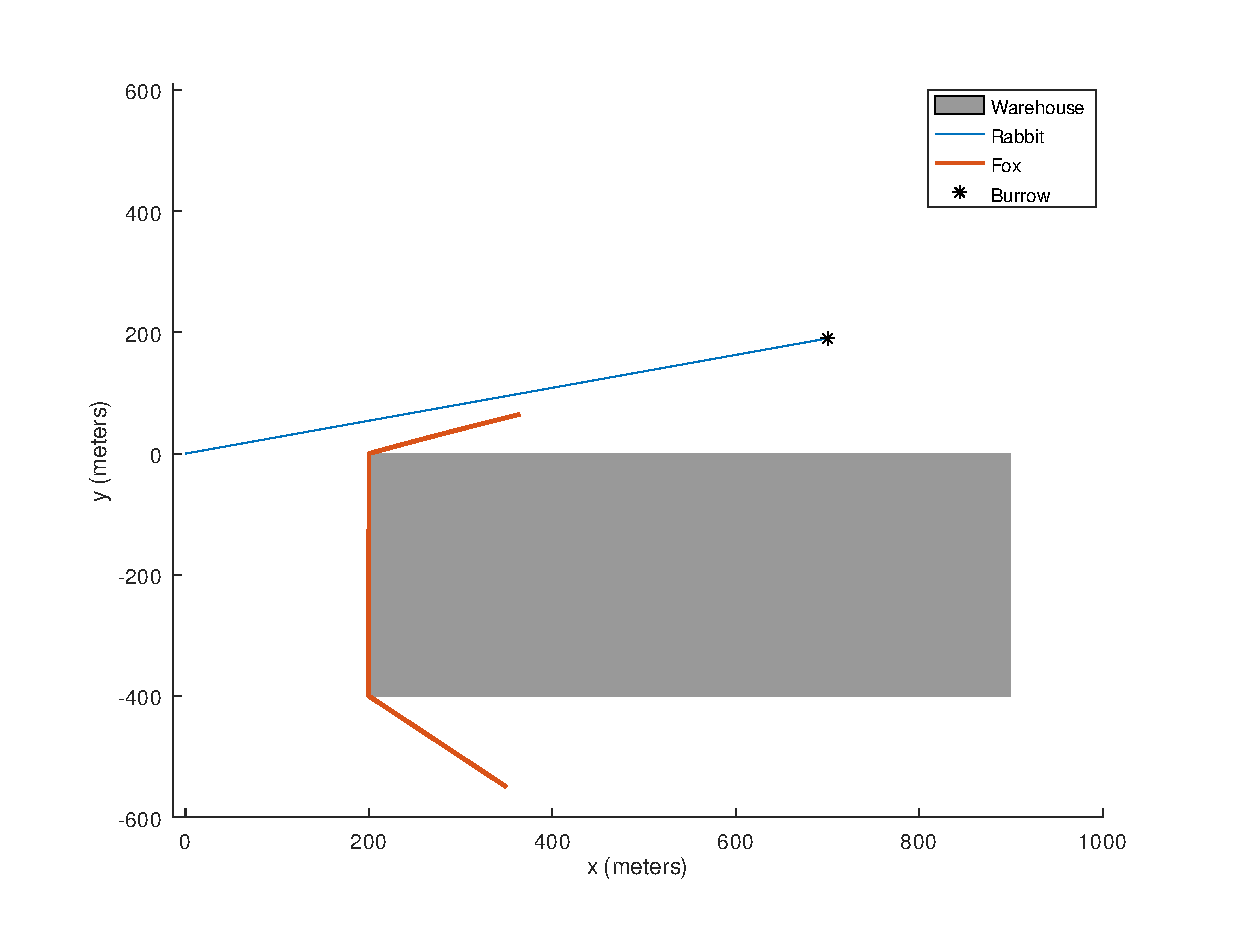
\includegraphics[scale=0.5]{realisticModel.eps}

      \label{fig:realisticModel}
\end{figure}





